\chapter{Technical Architecture}
\vspace*{-2ex}

\section{Preparing Data: DataLoader} \label{dataloader}

For the scope of this project, the data acquired was in the form of text-only English news articles, pertaining to the airline industry. This data was provided by Deep Search Labs (DSL) as a collection of news articles scraped from Bloomberg News, containing information such as the url of news article, the date it was published, the headline (title), the author, a pre-processed category and the article itself. The data (originally) a csv file, was loaded as a pandas dataframe for easy management and manipulation. An example of the format of the data is shown in~\Cref{dataframe}

\begin{figure}[H] 
\centering
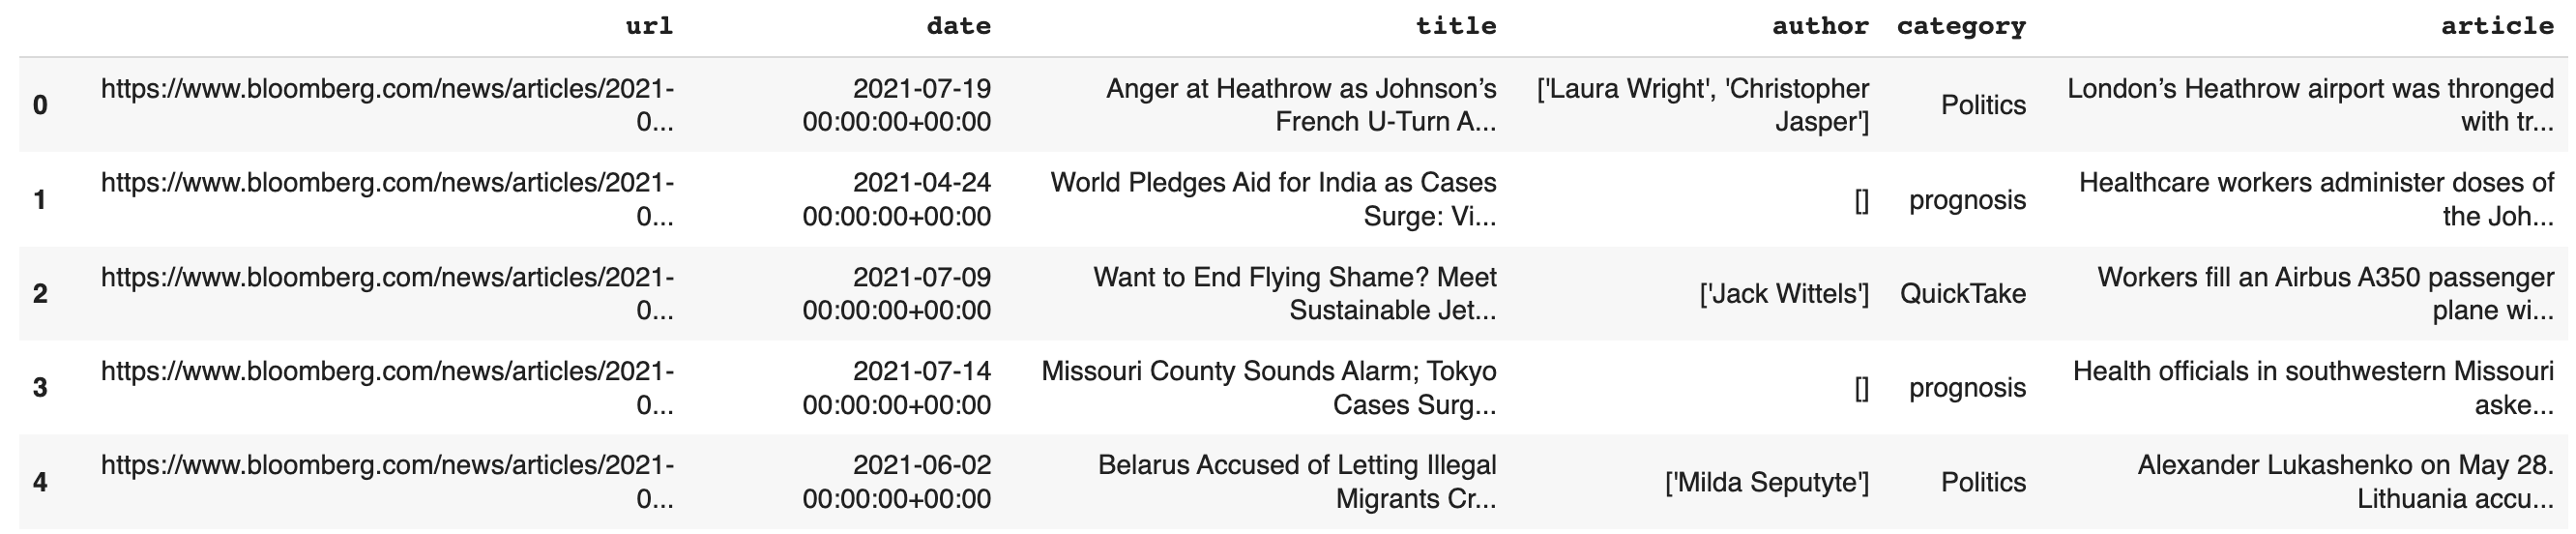
\includegraphics[width=0.8\linewidth]{images/dataframe.png}
\caption{Example data format}
\label{dataframe}
\end{figure}

The objective was to analyse the semantic information in the news articles for each category within a specific time interval. This prompted the need to divide the data meaningfully and was done by grouping the articles by time intervals of a year using the `date published' column as well the existing categories in the data to act as a control scaffold. Therefore, an input data group consisted of the articles in a specific category (e.g. Business) during a specific time interval (e.g. 2021). The motivation behind this was to see how news in certain categories changes over time in terms of topics extracted as well as information derived from semantic triples within these topics.

Once these '(Year, Category)' groups were obtained, they were filtered based on their size (i.e., the number of member articles) by omitting all those whose size was less than the $| mean - standard \ deviation |$ of the size of all groups. The reason for using the absolute difference between the mean and standard deviation of the value counts (size) of the groups was because variance in the sizes of groups was too high. Therefore, the aim was to retain the larger year-category groups but omit the extremely small groups. This ensured that the input data was of a significant size in order to yield relevant results before any further processing was done.  

% architecture overview
\section{System Design}

\begin{figure}[H]
\centering
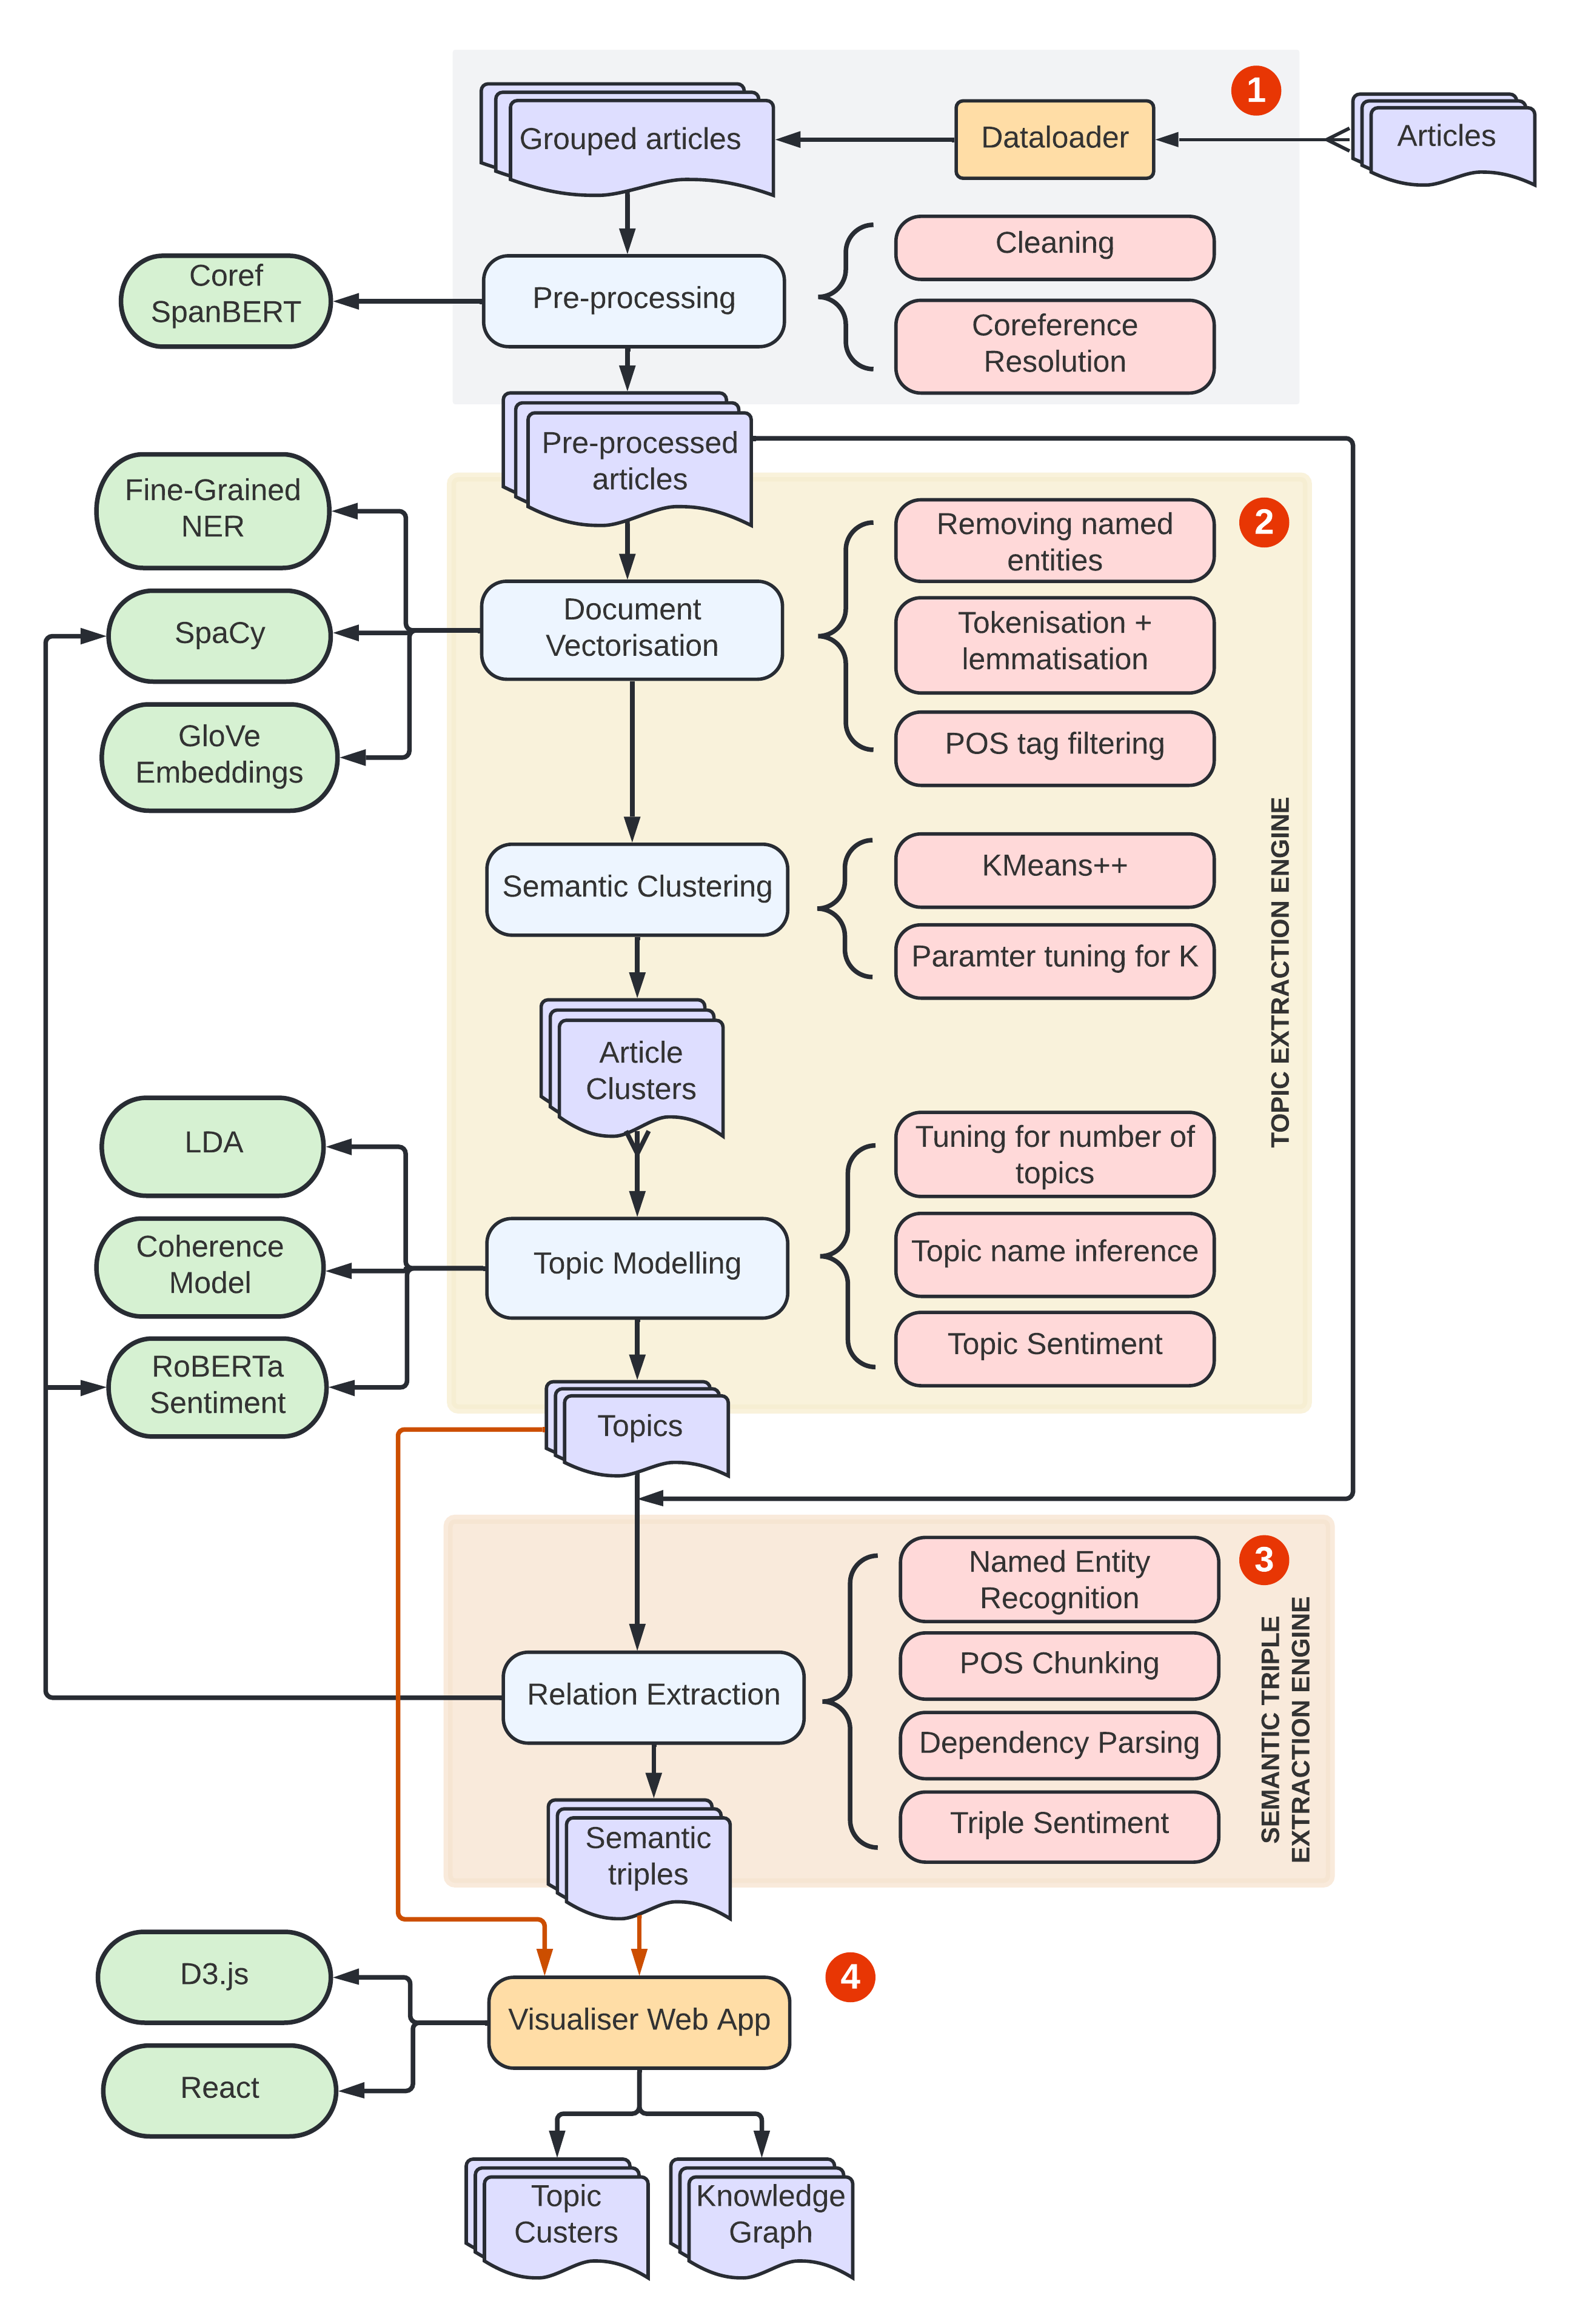
\includegraphics[width=0.8\linewidth]{images/system_arch.png}
\caption{System Architecture Diagram}
\label{fig:sys_arch}
\end{figure}
At a high level, the tool's main goal is to perform semantic analysis on the news corpora to extract information such as topics and semantic triples from the articles.~\Cref{fig:sys_arch}, shows a high level architecture diagram which follows the pipeline of the semantic analyser tool which follows 4 key stages: 

% of loading data, passing the input groups to the topic extraction engine, using the output latent topics as input for the semantic triple extraction engine, and finally, displaying the outputs from these engines as graphs in a web application. 

\begin{enumerate}
    \item \textbf{Data preparation:} The year-category data groups are generated from the dataset by the \texttt{dataloader} as discussed in~\Cref{dataloader}. Each input data group then follows the pipeline of pre-processing $\rightarrow$ topic extraction $\rightarrow$ semantic triple extraction engine. 
    
    \item \textbf{Topic Extraction Engine:} This involves semantic clustering of the articles, from which latent topics are extracted. These topics undergo processing such as topic name inference, keyword extraction and sentiment analysis to obtain semantic information about these topics.
    
    \item \textbf{Semantic Triple Extraction Engine:} For each topic in a semantic cluster, this engine extracts triples of type subject-predicate-object from sentences in articles associated with the topic. Each triple corresponds to an article and is accompanied by its sentiment.
    
    \item \textbf{Visualisation App:} Finally, the semantic clustering and latent topic models are visualised using circle packing graphs and the semantic triples are visualised using a force directed graph developed using D3.js. 
    

\end{enumerate}
\section{Technologies used}
\vspace{-1ex}
\subsection{Libraries} \label{libraries}

\textbf{SpaCy} is an open-source NLP library ``designed specifically for production use"~\cite{spacy}. It uses state-of-the-art pre-trained models and in-built pipelines for data processing techniques such as tokenisation, dependency parsing, POS tagging etc. The motivation for using this over other alternatives such as NLTK, was that it was much faster than NLTK for word tokenisation and POS-tagging. Additionally, the NLTK API is quite primitive in comparison to the object-oriented spaCy and requires a lot of unnecessary string manipulation~\cite{spacy-nltk}. The spaCy pipeline is trained on several models. For this project, the pre-trained English en-core-web-lg model was used with a large word vector table with approximately 500,000 entries~\cite{spacy}.  

\textbf{Gensim} is an NLP open-source library that makes use of state-of-the-art models for word vectorisation, text similarity and topic modelling. For this project, this library was used for the pre-trained models it exposes, in particular, \texttt{Word2Vec} and \texttt{GloVe} as well as the Latent Dirichlet Allocation (LDA) model used for topic modelling. 

\textbf{AllenNLP} is an open-source NLP library built on PyTorch and offers a variety of well-engineered existing state-of-the-art model implementations~\cite{allennlp}. Additionally, it is well integrated with components from the spaCy library such as the \texttt{Tokeniser} and \texttt{SentenceSplitter}, making it a fitting choice for this project. 

\textbf{D3.js} is a JavaScript library used for building data visualisations in the web browser. This was used in conjunction with React to build the web application for the visualisation tool. The motivation for using this library over other alternatives was it's data-driven approach to DOM manipulation which enables building customisable interactive visualisation frameworks. 

% \textbf{Ray} is an easy-to-use, fast distributed execution framework. It is designed to scale programs using state of the art ML libraries. This was used over the Python multiprocessing library as this provides a clean way to store memory intensive models in shared memory and run the functions tagged remote asynchronously giving a major performance gain.

\subsection{Models} \label{s:models}

Given the extensive prior research in literary analysis and natural language processing, the decision was made to use some of the state-of-art pre-trained models which have proven to be useful in other domains for this problem. The models used in different parts of the project are as follows: 

\textbf{SpanBERT for Coreference Resolution} is a state-of-the-art model used for co-reference resolution developed by the Allen Institute of Technology. It uses the SpanBERT embeddings to get ``high-order coarse-to-fine'' predictions of spans of text~\cite{spanBERT}. The motivation for using this over its predecessor BERT was that SpanBERT outperforms it for the coreference resolution task as it masks random contiguous spans of text unlike BERT which masks random tokens in a sequence, resulting in improved span predictions. The model scores these predictions to get coreference clusters which are applied to get the resolved text~\cite{spanBERT}.

\textbf{RoBERTa Stanford Sentiment Treebank} is a binary classifier trained on RoBERTa large for the Stanford Sentiment Treebank dataset, on which it achieved 95.11\% accuracy~\cite{roberta}. RoBERTa is another variant of BERT and stands for a Robustly Optimised BERT approach. Where BERT is optimised for Masked Language Model task (MLM) and Next Sentence Prediction (NSP), RoBERTa forgoes the latter and only minimises the loss for MLM, in which the model predicts `masked' (hidden) words by learning their representation using words occurring to the left and right of the `masked' word in the sentence (bi-directional). RoBERTa uses dynamic masking (i.e., different parts of the sentence are masked for each epoch), unlike BERT, which uses static masking (i.e., the same parts of the sentence are masked each epoch)~\cite{roberta}. 

\textbf{Fine-Grained NER} is a state of the art named entity recognition model from AllenNLP and is a re-implementation of the Lample (2016)~\cite{lample} model. It makes use of bi-direction LTSM with a Conditional Random Field layer (CRF) and uses two types of embeddings: character embeddings and ELMo embeddings (See~\Crefrange{named_ents}{elmo}). In this paper~\cite{lample}, a comparison study for the performance of the model for English NER on the CoNLL-2003 test set highlights that it outperforms several other models giving an F1 score of 90.94\%~\cite{lample}. The motivation for using this model was this high accuracy and that the model identifies a broad range of 16 semantic types (See Appendix~\Cref{appendix:semantic_types}).

\section{Visualisation Web Tool}
As an extension to the core body of work done including semantic clustering, latent topic model extraction (done by Topic Extraction Engine) and inferring semantic triples (done by Semantic Triple Extraction Engine), an interactive visualisation pipeline was created to display the results from these two engines in the semantic analysis tool. 
This was done by developing a web interface using React and D3.js to build stateful cohesive visualisations, allowing the integration of all the different results in a web application. In the latter stages of the project, the application was hosted on Heroku~\cite{heroku} as a scalable approach to accommodate user testing and evaluation discussed in~\Cref{s:user_eval}. This tool adopted the principals of visualisations discussed in~\Cref{principal_vis} such as incorporating user interactivity and an intuitive consistent layout with labelled information.